\documentclass[a4paper]{proc}

\usepackage[utf8]{inputenc}
\usepackage[T1]{fontenc}
\usepackage[english]{babel}
\usepackage{graphicx}
\usepackage{url}
\usepackage{mathtools}

\author{Paul MABILEAU\\\texttt{paul.mabileau@telecom-sudparis.eu} \and Franck STAUFFER\\\texttt{franck.stauffer@telecom-sudparis.eu}}
\title{\textbf{Recursive Inter-Network Architecture's Security}}

\begin{document}
\maketitle
\tableofcontents
\newpage
\part{Introduction}
The Recursive Inter-Network Architecture (RINA) is a network architecture born in John Day's \texttt{Patterns in Network Architecture: A Return to Fundamentals} in 2008.
It emerges from the fact that TCP/IP was designed a while ago without security in mind and that the huge amount of RFCs\cite{rfc} published since 1969 by the IETF to add security in it created complexity.\cite{assessing-security}
Moreover the book states that the current internet architecture is not an actual `inter-net' but more a juxtaposition of different networks on a same bigger network.
\\To remedy, it proposes to go back to fundamentals and states that networking is only Inter Process Communication (IPC) and thus John Day proposed the Recursive InterNetwork Architecture (RINA) as an alternative.
RINA promises to reduce complexity by reducing the number of protocols, separating mechanisms and policies, using connection-less communications and reworking the whole way things work.
This architecture claims to be more secure by design than the TCP/IP architecture.
\\The architecture is also developped by the Pouzin Society\cite{psoc} that kind of replace the IETF by publishing specifications.
Some simulations and studies have been lead in Europe with IRATI\cite{web:irati} and PRISTINE\cite{pristine} for example.
You can also find a framework to test RINA on OMNeT++ named RINASim at \url{https://rinasim.omnetpp.org/}.
\\First we will provide a presentation of the RINA architecture, then we will discuss its security compared to the TCP/IP architecture.
\newpage

\part{Comparing RINA and TCP/IP}
\section{Architecture}
RINA uses a single recursive layer named a Distributed IPC Facility (DIF). It can be stacked as much as needed by the network architecture instead of being a static model like in TCP/IP\@.
Inside the DIFs there are IPC Processes (IPCPs) that communication using a Common Distributed Application Protocol (CDAP) that only allows six basic operations to be used on a remote object\cite{wiki}:
\begin{itemize}
    \item Create
    \item Delete
    \item Read
    \item Start
    \item Stop
    \item Write
\end{itemize}
Those IPCPs deal with tasks which can be divided in three parts (figure~\ref{fig:arch}).
The parts are ordered from the less complex and more frequent to the more complex and less frequent ones:
\begin{itemize}
    \item Data Transfer: it deals with SDU delimiting (fragmentation, concatenation, separationm, reassembly), SDU Protection (integrity/error detection), Relaying and Multiplexing Task and actual Data Transfer\cite{irati}
    \item Data Transfer Control: it deals with Transmission Control, Retransmission Control and Flow Control
    \item Layer Management: it deals with Authentication, Enrollment, Namespace Management, Flow Allocation, Forwarding Table Generator, Resource Allocation, Security Management and CDAP Parsing and Generation
\end{itemize}
The $N-DIF$ only knows $(N + 1)-DIF$ and $(N - 1)-DIF$\@.
The $(N + 1)-DIF$ is saw as an Application Process (AP) because all IPCPs are actually APs.
There is one exception to this rule, there is a special DIF that is called a Distributed Application Facility (DAF) that has no $(N + 1)-DIF$\@.
This DIF is composed of one or more Distributed Application Processes (DAPs) in place of IPCPs.
This DIF can be considered as the Application layer from the TCP/IP model.
IPCPs only communicates with other IPCPs in the same DIF like in the TCP/IP model with layers.
IPCs communicate in the form of Protocol Data Units (PDUs) that contain a header or a trailer (named Protocol Control Information (PCI)), and a payload.\cite{PINS}
The DIFs choose to use a connection-oriented or a connection-less communication depending on the needs of the IPCP\@.

\begin{figure}
    \centering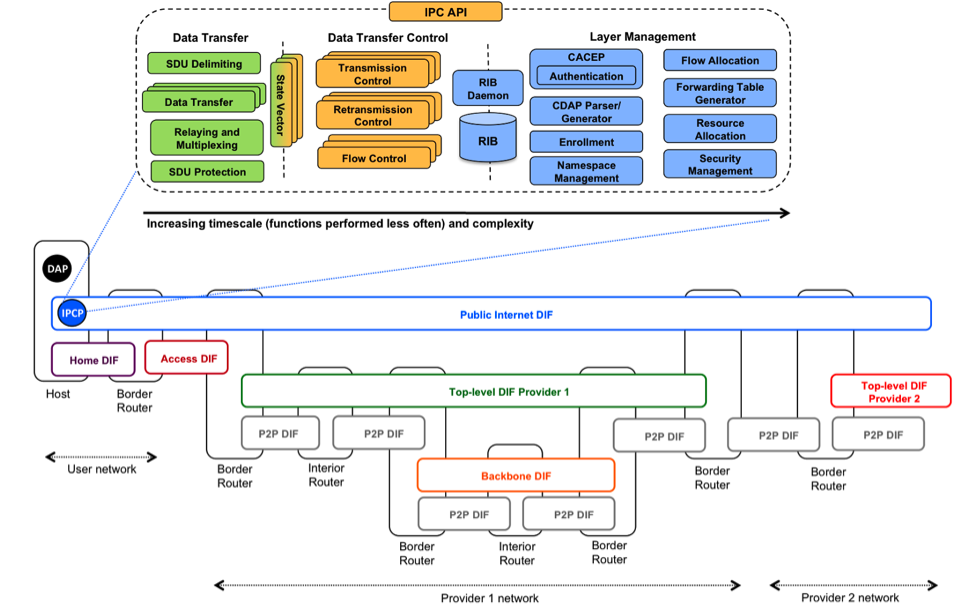
\includegraphics[width=\columnwidth]{arch.png}\caption{RINA's architecture}\label{fig:arch}
\end{figure}

\section{Delta-t synchronization}
According to RINASim's webpage: `There is no need for explicit state synchronization (hard-state) and tools like SYNs and FINs are unnecessary'.
Instead they use the Delta-t transport protocol\cite{65288}.
It is a time-based synchronization techniques that only needs 3 timers:
\begin{itemize}
    \item Maximum Packet Lifetime
    \item Maximum time to attempt retransmission
    \item Maximum time before Acknowledgement
\end{itemize}
In this protocol, every connections exists at every point in time.
When there is no traffic the synchronization state is maintained during 2 or 3 Maximum Packet Lifetimes.\cite{rinasim}

\part{Security provided by RINA's conception}

\part{(optionnel) The threats to RINA}

\nocite{*}
\newpage
\bibliographystyle{unsrt}
\bibliography{report}
\end{document}
